% Chapter Template

\chapter{L'algoritmo H265} % Main chapter title

\label{Chapter4} % Change X to a consecutive number; for referencing this chapter elsewhere, use \ref{ChapterX}

\lhead{Capitolo 4. \emph{L'algoritmo H265}} % Change X to a consecutive number; this is for the header on each page - perhaps a shortened title

%-------------------------------------------------------------------------------
%	SECTION 1
%-------------------------------------------------------------------------------

\section{Suddivisione in blocchi dell'immagine} 
Un'immagine viene inizialmente suddivisa in \emph{coding tree unit} (CTU), di 
forma quadrata e dimensione costante per tutta la sequenza video: 64x64, 32x32 
o 16x16 pixel. Questa ``flessibilità'' nella dimensione del blocco fondamentale 
della suddivisione è stata introdotta da HEVC, in quanto tutti i suoi 
predecessori utilizzano un \emph{macroblocco} di 16x16 pixel; ciò permette a 
HEVC di sapersi adattare meglio a -e comprimere maggiormente- video di diverse 
dimensioni.
Il CTU è un'unità logica che consiste di tre ulteriori blocchi: Luma, 
ChromaB e ChromaR (Y, Cb e Cr). Ognuno di questi blocchi è un 
\emph{coding tree block} (CTB), ed è della stessa dimensione relativa 
del CTU, sebbene la dimensione effettiva di ogni blocco sia regolata dal 
\emph{chroma sampling format}: se il formato fosse 4:2:0, tipico di questi 
encoding, il blocco Y sarebbe 64x64 pixel, mentre i due blocchi di crominanza 
risulterebbero di 32x32 pixel. Quando un blocco risulta più piccolo del 
CTU di partenza (in questo caso, e quasi sempre, i due di crominanza) 
subisce un \emph{upscaling}: questo comporta una minore definizione e una 
maggiore compressione dell'immagine finale, resa ammissibile dalla maggiore 
sensibilità dell'apparato visivo umano alla luminanza rispetto al colore.
\begin{figure}[H]
  \centering
    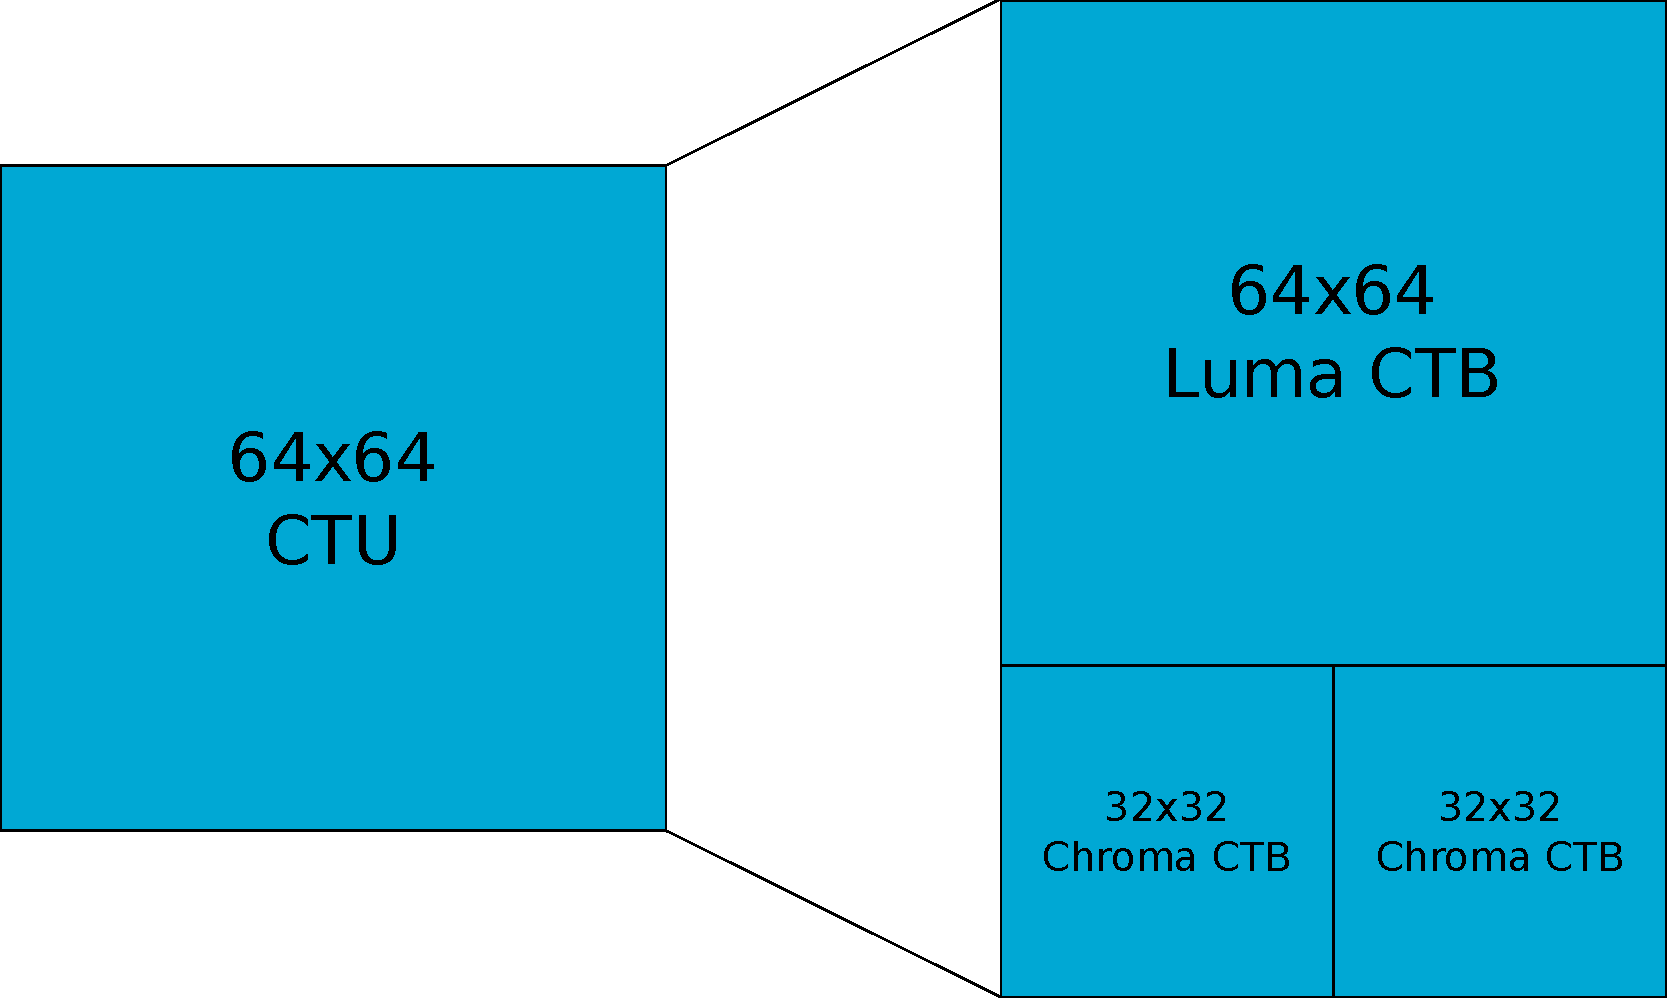
\includegraphics[scale=0.20]{Figures/CTU-CTB}
  \caption{Suddivisione del CTU in CTB}
\end{figure}
// Rivedere questo paragrafo: ovunque viene detto che il CTB è suddiviso \\
// in CU. \\
Il CTB può essere ulteriormente suddiviso in \emph{coding blocks} (CB), che 
sono il punto in cui viene decisa quale tipo di \emph{prediction} utilizzare.
Supponendo di avere un CTB di dimensione 64x64 la suddivisione può essere 
effettuata con CB grandi 64x64, 32x32, 16x16 o 8x8, ottenendo una struttura
detta \emph{quad-tree}, in cui il CTB è suddiviso ricorsivamente. 
Il CB, così come il CTB, consiste ancora nei tre blocchi Y, Cb e 
Cr, che definiscono un \emph{coding unit} (CU), ovverò l'unità in cui viene 
codificato il tipo di predizione. La scelta di quest'ultima è autonoma per ogni 
CU.
\begin{figure}[H]
  \centering
  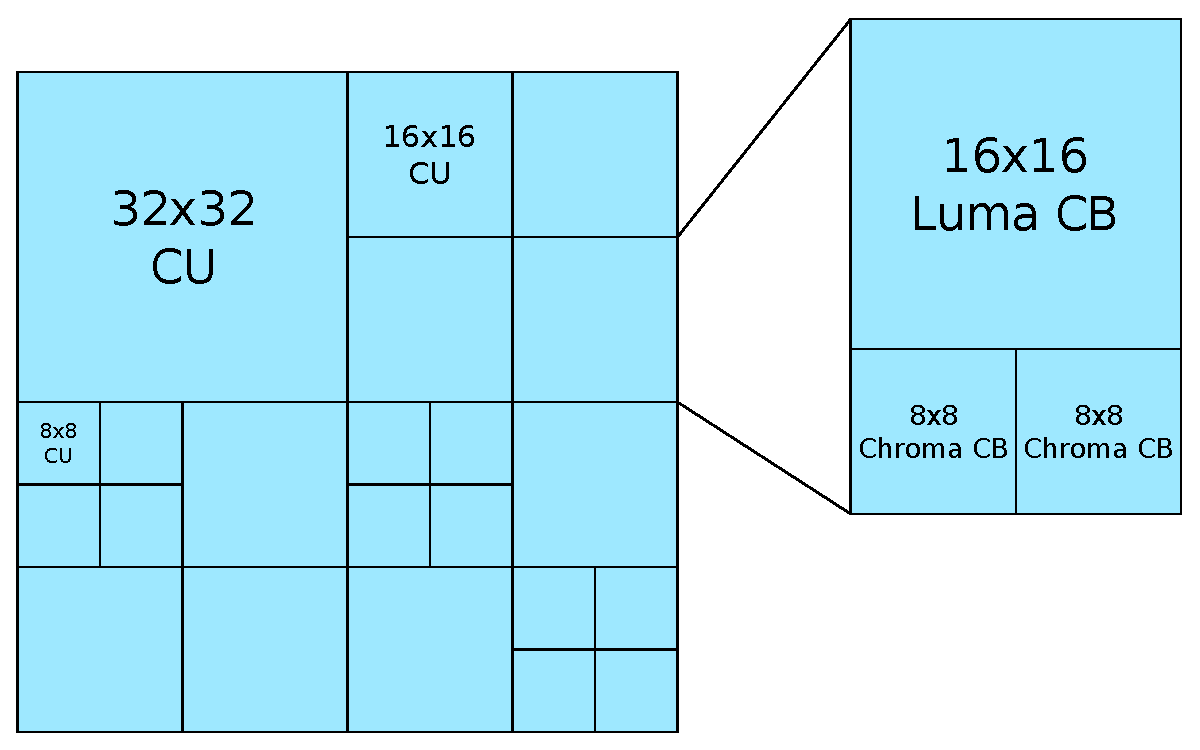
\includegraphics[scale=0.50]{Figures/CTB-CU-CB}
  \caption[Suddivisione del CTB in CU]{Suddivisione di un CTB 64x64 in una 
struttura a \emph{quadtree}}
\end{figure}
In caso ci sia bisogno di una maggiore precisione nella predizione (e.g., 
oggetti minuscoli che si muovono in un CB 8x8) è possibile suddividere i
\emph{coding block} in \emph{prediction block} (PB), che, in caso di 
\emph{inter prediction}, possono non seguire la struttura a \emph{quadtree} dei
blocchi precedenti:
\begin{figure}[H]
  \centering
  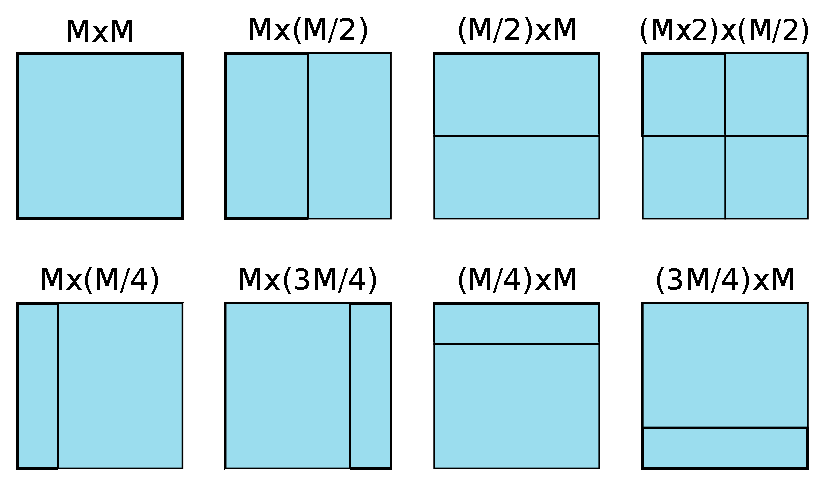
\includegraphics[scale=0.50]{Figures/PB}
  \caption{Possibili strutture di un \emph{prediction block}}
\end{figure}
Un PB definisce una regione che, per effettuare una predizione, utilizza gli 
stessi parametri di movimento: il numero di ipotesi di movimento (che può 
valere uno o due a seconda che si usi l'immagine precedente o quest'ultima 
e le successiva per cercare il blocco che si è mosso) e, per ognuna di queste, 
l'indice dell'immagine di riferimento e il vettore di movimento.
L'insieme dei tre PB, che possiedono lo stesso tipo di suddivisione, 
forma una \emph{prediction unit} (PU).
Per effettuare la codifica del segnale di errore un CB viene suddiviso in 
\emph{transform block}, dando forma ad una struttura a \emph{quadtree} che 
viene chiamata \emph{residual quadtree} (RQT); solitamente la suddivisione 
è mantenuta uguale per i TB Luma e Chroma.
%-------------------------------------------------------------------------------
%	SECTION 2
%-------------------------------------------------------------------------------
\section{Intra prediction}
Su un blocco di campioni contigui che possiedono gli stessi parametri 
predittivi, siano essi CB o PB, verrà eseguita la stessa 
\emph{intra prediction}.
Di quest'ultima esistono due tipologie a seconda delle caratteristiche 
del blocco: in caso di figure e strutture geometriche sarà utilizzata 
la \emph{angular prediction}, viceversa, se la predizione viene eseguita 
su contenuti meno strutturati, sarà eseguita una \emph{planar + DC prediction}. 
In entrambi i casi, la predizione si basa sui campioni contigui (o 
\emph{neighbour}) al blocco che si trovano a sinistra e a destra di 
quest'ultimo.

\paragraph*{Pre-filtering}
Prima di effettuare una delle due predizioni è possibile eseguire uno 
\emph{smoothing filter} sui campioni di riferimento, che dipende dal tipo di 
predizione che verrà successivamente eseguita. Le due possibilità sono le 
seguenti:
\begin{enumerate}
\item Un semplice \emph{lowpass filter} lineare con risposta all'impulso 
[1 2 1]/4 (a)
\item Se la dimensione del TB è 32x32 e i campioni di riferimento sono 
abbastanza ``morbidi'', questi vengono sostituiti con le corrispondenti 
interpolazioni lineari dei cambioni agli estremi (b)
\end{enumerate}

\begin{figure}[H]
  \centering
  \begin{tabular}{cc}
    \subfloat[]{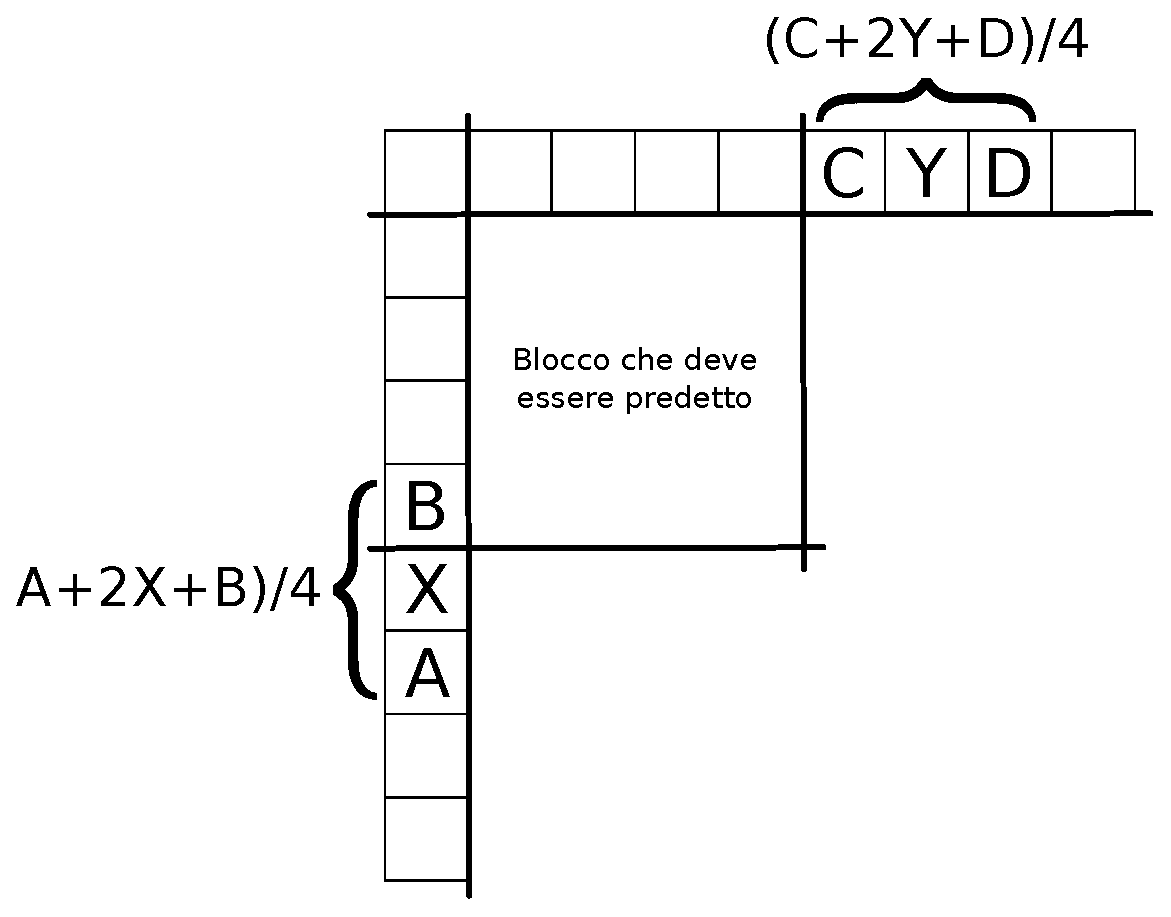
\includegraphics[scale=.35]{Figures/Filtering_a}}
    &
    \subfloat[]{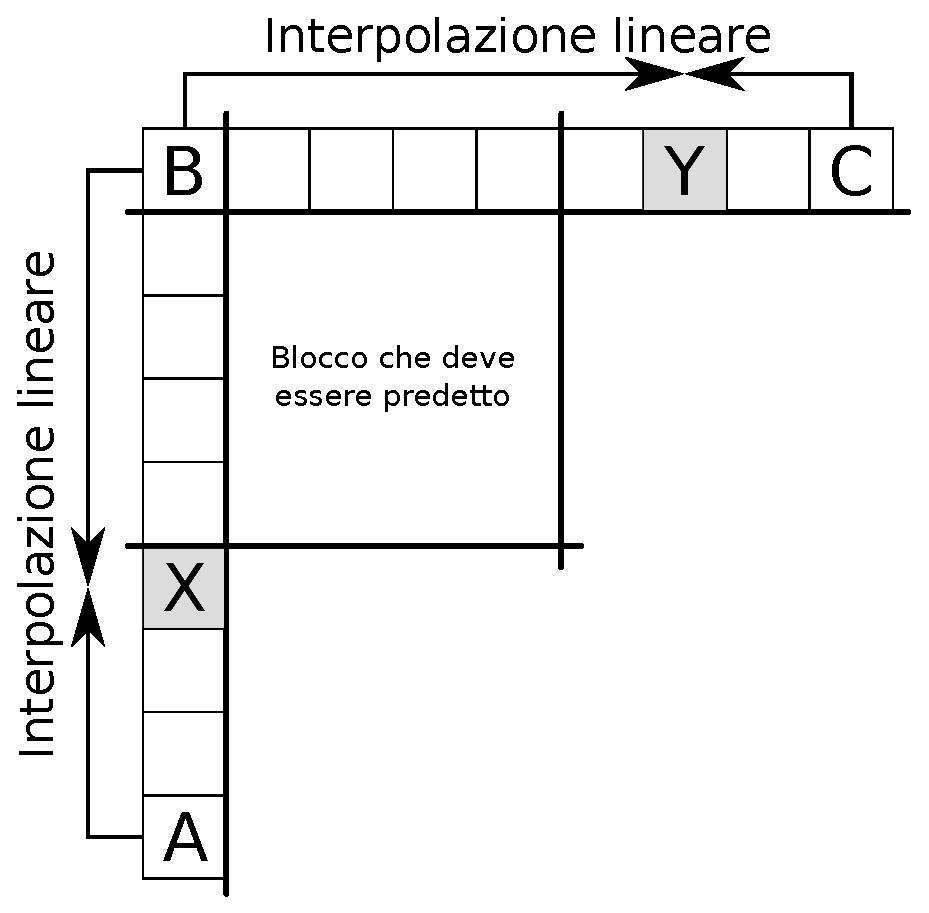
\includegraphics[scale=.35]{Figures/Filtering_b}}
  \end{tabular}
  \caption{I due diversi tipi di \emph{pre-filtering}}
\end{figure}
%-----------------------------------
%       SUBSECTION 1
%-----------------------------------

\subsection{Angular prediction}
Per la predizione angolare l'encoder deve scegliere uno tra 33 possibili angoli:
 questo tipo di predizione stima in modo accurato le strutture direzionali che 
sono tipicamente presenti nelle foto, tra cui le più frequenti risultano essere
 quelle orizzontali e verticali.
Per far fronte a quest'ultima circostanza, H.265 predispone gli angoli in modo 
che siano presenti in numero maggiore intorno alle due direzioni più frequenti;
 il numero totale di angoli e la loro disposizione è il risultato della ricerca 
di un buon \emph{trade-off} tra qualità e complessità computazionale 
dell'encoder.
\\
// Immagine qui
\\
Gli angoli prendono il nome di ``modi predittivi'' (\emph{prediction modes}) e 
il loro raggruppamento è diviso tra orizzontali e verticali.
Nell'immagine di cui sopra si può notare come gli angoli ``orizzontali'' siano 
quelli il cui segmento ha la sua origine in un campione collocato a sinistra, 
mentre l'origine del segmento degli angoli ``verticali'' risiede in un campione 
posizionato in alto.\\
Il parametro angolare $A$ indica la posizione, in termini di campioni, rispetto 
al campione centrale (che ha valore $0$).
Utilizzando il raggruppamento e il parametro $A$ è possibile identificare 
univocamente un modo predittivo; prendendo nuovamente in esame l'immagine la 
sigla $H+2$ corrisponde al modo predittivo 9, la sigla $H-2$ al modo predittivo 
11 e così via.\\
Per effettuare le predizioni dei campioni di un blocco viene prima costruito, 
per comodità, un array che contiene i campioni di riferimento riposizionati 
nell'ordine che risulta più conveniente per il modo predittivo scelto; infatti 
ogni campione $p[x][y]$ da predire viene ottenuto mediante l'interpolazione dei 
due campioni contigui all'interno dell'array di riferimento, con il fattore di 
interpolazione che risulta essere proporzionale all'angolo -o modo predittivo- 
selezionato.
%-----------------------------------
%       SUBSECTION 2
%-----------------------------------

\subsection{DC + Planar prediction }
\paragraph*{DC} La predizione DC prevede un valore costante per tutto il 
blocco, determinato dalla media dei valori dei campioni di riferimento che si 
trovano sopra e a sinistra del blocco.

\paragraph*{Planar} La predizione ``planare'' genera un blocco che presenta 
colori morbidi e privi di discontinuità marcate anche ai bordi. Questo è 
ottenuto tramite una semplice interpolazione, punto per punto, dei campioni di 
riferimento (evidenziati in giallo) con i loro estremi (evidenziati in grigio):
\begin{align*}
p[x][y] = 
%\left
[&\fcolorbox{yellow}{white}{$(N-1-x)*p(-1,y)$}+
  \fcolorbox{black!50}{white}{$(x+1)*p(N,-1)$}+\\
 &\fcolorbox{yellow}{white}{$(N-1-y)*p(x,-1)$}+
  \fcolorbox{black!50}{white}{$(y+1)*p(-1,N)$}+N] \gg log_2(N+1)
%\right]
\end{align*} 
dove $NxN$ è la dimensione del TB.
\\
// Inserire immagine
\\ 
L'immagine mostra come il risultato (c) sia la media di due interpolazioni: una 
orizzontale (a) e una verticale (b).
%-----------------------------------
%       SUBSECTION 3
%-----------------------------------

\subsection{Post-filtering}
Esistono tre casi in cui è necessario eseguire anche un filtraggio successivo, 
tipicamente quelli in cui si presentano brusche discontinuità ai bordi, e sono 
gli \emph{angular mode} esattamente orizzontali e verticali e la 
\emph{DC prediction}.
Il fatto che venga eseguito in sole tre evenienze è determinato dalla volontà 
di limitare la complessità computazionale di fronte a svantaggi che possono 
risultare  marginali, come nel caso delle predizioni diagonali, e dalla ricerca 
di un buon rapporto tra qualità e precedente complessità.
In seguito a test sperimentali è stato notato che le predizioni dei canali 
Chroma risultano sempre relativamente morbide; conseguentemente questo 
filtraggio viene eseguito solo sui canali Luma, e consiste nella modifica dei 
pixel ai bordi all'interno del blocco, secondo le seguenti modalità:
\begin{enumerate}
\item \emph{Angular prediction}, angolo verticale: \\
\begin{align*}
p(0,y)\mathrel{+}=\left(\frac{p*(-1,y)-p*(-1,-1)}{2}\right) 
\forall y \in {[0,N-1]}
\end{align*}

\item \emph{Angular prediction}, angolo orizzontale: \\
\begin{align*}
p(x,0)\mathrel{+}=\left(\frac{p*(x,-1)-p*(-1,-1)}{2}\right) 
\forall x \in {[0,N-1]}
\end{align*}

\item{ \emph{DC prediction}, posto $dcVal$ il valore della posizione: \\
\begin{align*}
p(0,0)=(p*(-1,0)+2dcVal+p*(0,-1)+2)*4
\end{align*}

Con i campioni ai bordi filtrati nel seguente modo:
\begin{align*}
p(x,0)&=(p*(x,-1)+3dcVal+2)*4 \forall y \in {[0,N-1]} \\
p(0,y)&=(p*(-1,y)+3dcVal+2)*4 \forall y \in {[0,N-1]}
\end{align*}

Dove $dcVal \in {[0,1]}$
}
\end{enumerate}

L'immagine seguente mostra un esempio di CTB Luma interamente predetto intra: \\

// Inserire immagine
%-------------------------------------------------------------------------------
%       SECTION 3
%-------------------------------------------------------------------------------

\section{Inter Prediction}
L'\emph{inter prediction} sfrutta la correlazione temporale dei frame per 
ottenere una \emph{motion compensated prediction} (MCP), ovvero un PB predetto 
a partire da PB ``predittori'' che appartegono a frame precedentemente 
decodificati, supponendo che nel PB predetto essi siano traslati: 
\\
// Inserire immagine
\\
Per ogni PB l'encoder ricava un vettore ${(\Delta x,\Delta y,\Delta t)}$ 
chiamato \emph{motion data}, dove ${(\Delta x,\Delta y)}$ è il 
\emph{motion vector} e indica la traslazione compiuta dal PB in questione, 
mentre ${(\Delta t)}$ è l'indice temporale dell'immagine a cui appartiene il PB 
predittore.
È anche possibile effettuare una ``bipredizione'': in questo caso si usano 
due \emph{motion data} ottenendo due MCP di cui viene ricavata la media (che 
può anche essere pesata) per ottenere il risultato, come illustra la figura 
precedente.
\\
Viene inoltre sfruttata la correlazione spaziale (ma sempre legata al tempo) 
dei \emph{motion vector}, basata sulla supposizione che i \emph{motion vector} 
relativi a PB spazialmente vicini non differiscano eccessivamente, eccezion 
fatta per eventuali punti di discontinuità come i cambi di oggetto. È inoltre 
ipotizzata una discreta continuità nel tempo per quanto riguarda i movimenti 
dell'intero \emph{frame}, escludendo variazioni brusche come i cambi di scena.
\\
Tutto questo viene tradotto nel concetto di \emph{motion vector predictor} 
(MVP); invece di trasmettere un \emph{motion vector} per ogni PB l'encoder 
trasmette l'errore o la \emph{motion vector difference} (MVD), tra quello 
predetto a partire da blocchi spazialmente o temporalmente contigui e quello 
normalmente calcolato con $MVD=MV-MP$.
Il decoder riceve la MVD e la sintassi necessaria a determinare il MVP (ovvero 
il tipo di predizione da utilizzare) e può dunque ricavare $MV$ come $MVD+MVP$.
 
Sebbene gli algoritmi che hanno preceduto H.265 (H.264, AVC) possiedano questo 
tipo di predizione, essi si limitano a calcolare $MVP$ come una media dei $MV$ 
vicini spazialmente: questa strategia non è più applicabile in HEVC a causa 
dell'elevata flessibilità delle strutture di predizione.
Il \emph{worst case scenario} presenta 16 $MV$ per lato da tenere in 
considerazione (come mostrato nell'immagine successiva), che porterebbe a 
complessità di codifica troppo elevate.

\begin{figure}[H]
  \captionsetup{justification=raggedright}
  \centering
  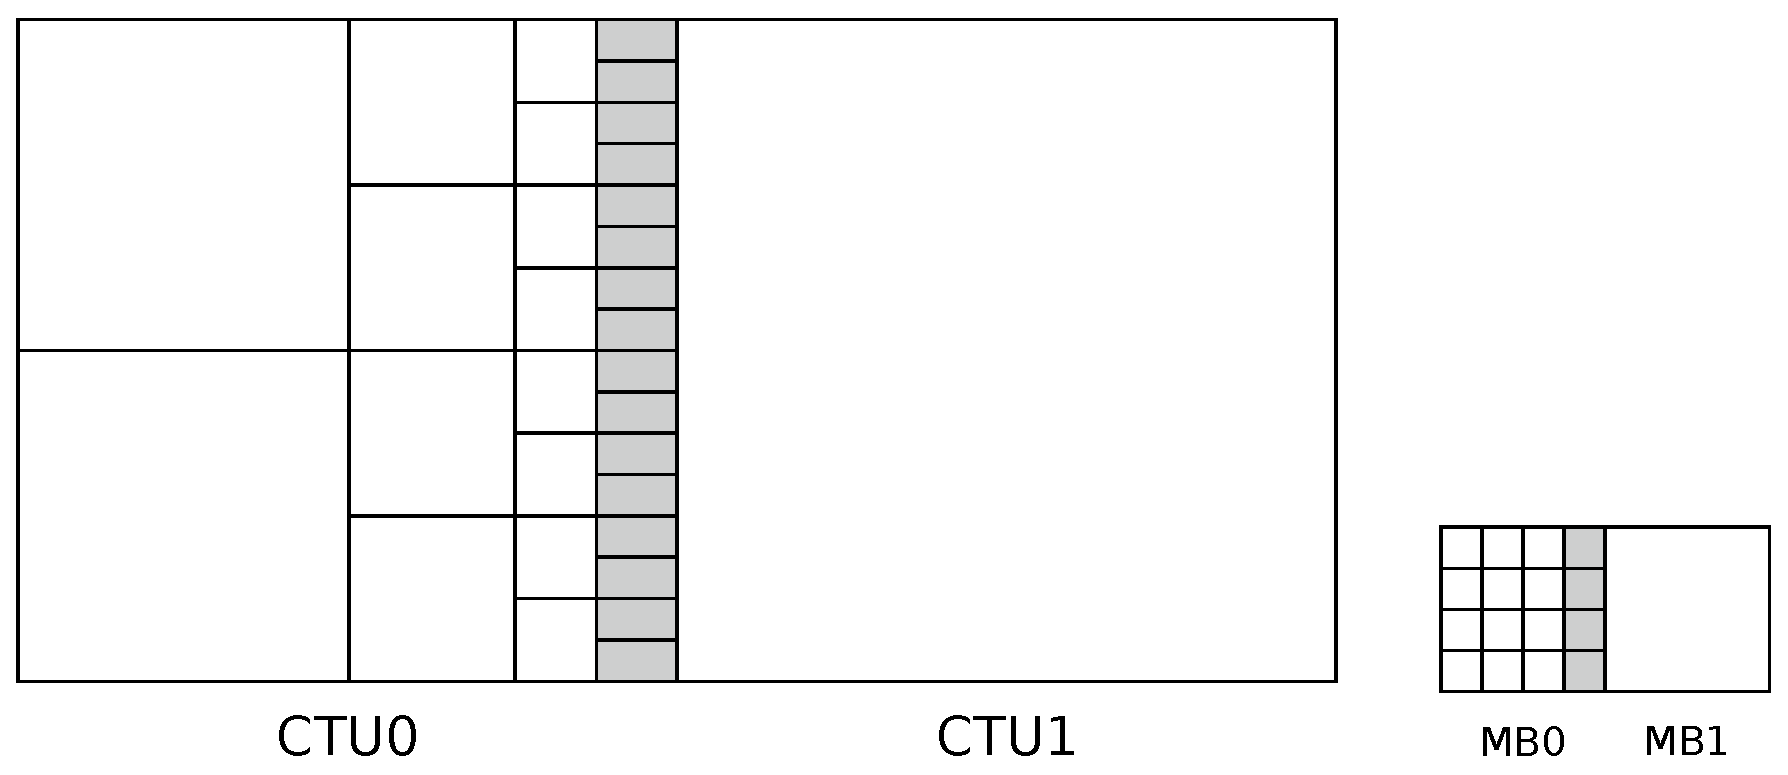
\includegraphics[scale=0.45]{Figures/Inter_pred_2}
  \begin{flushleft}
    \caption[Numero massimo di \emph{motion vector} in H.265 e H.264]
    {Numero massimo di \emph{motion vector} in H.265 (a sinistra) e H.264 \\
      (a destra). CTU0 possiede 16 PB Luma 8x4 contigui a CTU1 che è composto da
      un solo PB Luma 64x64. MB0 (\emph{Macro Block)} contiene quattro 
      partizioni di predizione 4x4 affiancate a MB1 che consta di una 
      partizione 16x16. }
  \end{flushleft}
\end{figure}

H.265 mette a disposizione un algoritmo per la costruzione di vettori 
\emph{candidate MVP} chiamato \emph{advanced motion vector prediction} (AMVP), 
ottenuto in seguito ad esperimenti esaustivi volti a trovare oredizioni che 
minimizzassero la complessità di codifica pur mantenendo buoni livelli di 
predizione (i.e., bassa entropia del segnale di errore MVD).\\
Una parte della sintassi di HEVC serve a comunicare al decoder quale MVP 
utilizzare tra quelli candidati, che sono due e scelti nei modi seguenti:
\begin{itemize}
\item Due \emph{spatial candidate} che derivano da cinque blocchi spazialmente 
vicini;
\item Viene tenuto come riserva un \emph{temporal candidate} derivato da due 
blocchi co-locati e temporalmente vicini:
\begin{itemize}
\item Nel caso che i due \emph{spatial candidate} siano uguali, o se uno di loro
 non sia disponibile, i due vettori candidati saranno uno spaziale e uno 
temporale;

\item Se entrambi i candidati spaziali non fossero disponibili, verrà 
considerato il vettore candidato temporale di riserva ed uno 
\emph{zero motion vector};

\item Nell'eventualità che sia i candidati spaziali sia i candidati temporali 
non siano disponibili, entrambi i candidati saranno \emph{zero motion vector}.
\end{itemize}
\end{itemize}

Gli \emph{spatial candidate} sono ottenuti prendendo in considerazione cinque 
blocchi spazialmente vicini suddivisi in due gruppi: il gruppo A contenente i 
due blocchi in basso a sinistra rispetto a quello che si vuole predire, il 
gruppo B con al suo interno tre blocchi in alto.
Generalmente, se i vettori dei blocchi considerati sono ricondicibili allo 
stesso \emph{reference id} (l'indice dell'immagine a cui fanno 
riferimento) di quello del blocco che si vuole predire, tali vettori saranno 
MVP.
Viceversa, MVP sarà il vettore scalato secondo una formula che dipende dalla 
differenza temporale dei \emph{reference id}.
Non sono invece presi in considerazione blocchi a destra o in basso dal 
momento che tali PB non sono ancora stati decodificati e non sono disponibili 
al decoder per la predizione.
\\
Per quanto concerne il \emph{temporal candidate} si lavora su una immagine 
co-locata e temporalmente vicina della quale, in fase di decodifica, si 
possiedono tutte le informazioni (ovvero un frame già decodificato); diversi 
esperimenti hanno dimostrato che i blocchi da prendere in considerazione sono 
due: quello al centro e quello in basso a destra rispettivamente alla posizione 
del blocco che si vuole predire.
Specificamente il vettore viene predetto utilizzando sempre il blocco in basso 
a destra, salvo la mancanza di disponibilità d quest'ultimo; ciò significa che 
esso risiede fuori dai bordi dell'immagine o viola vincoli imposti per motivi 
di memoria.
\newline \\
Infine HEVC risolve un problema legato alla struttura di suddivisione delle 
immagini \emph{quadtree}: quest'ultime permettono una grande flessibilità 
delle dimensioni dei blocchi con un basso costo di \emph{overhead} in termini 
di \emph{bit rate}. Per l'\emph{inter prediction} la struttura a \emph{quadtree}
 permette di suddividere minuziosamente quelle parti di immagine dhe presentano 
bruschi movimenti rispetto alle parti più statiche che non richiedono una 
grande informazione di movimento. Questo tipo di raggruppamento, tuttavia, 
origina facilmente bordi ineffettivi (\emph{over segmentation}); HEVC dispone 
di un  algoritmo di \emph{block merging} che consente di raggruppare PB con 
uguali parametri di predizione in modo da trasmetterne una sola copia.
\\
Nell'esempio mostrato dall'immagine seguente la parte a) è l'immagine 
originale, b) è l'immagine scomposta in PB secondo la struttura a 
\emph{quadtree} mentre c) mostra il risultato del \emph{block merging}.
\\
// Inserire immagine 
\\
%-------------------------------------------------------------------------------
%       SECTION 4
%-------------------------------------------------------------------------------

\section{Transform and Quantization}
Nel \emph{block-based video coding} i segnali di errore residui che derivano 
dalle predizioni intra o inter vengono trasformati e quantizzati prima di 
essere trasmessi.
Più nel dettaglio, un'immagine è suddivisa in blocchi quadrati di dimensione $NxN$, dove $N=2^M$ con $M \in \mathbb{N}$. Per ogni blocco esisterà un blocco 
residuo $U$ che verrà trasformato e quantizzato. \\
L'immagine mostra il percorso dei dati durante la fase di encoding (a) e 
di decoding (b):
\begin{figure}[H]
  \centering
  \begin{tabular}{cc}
    \subfloat[]{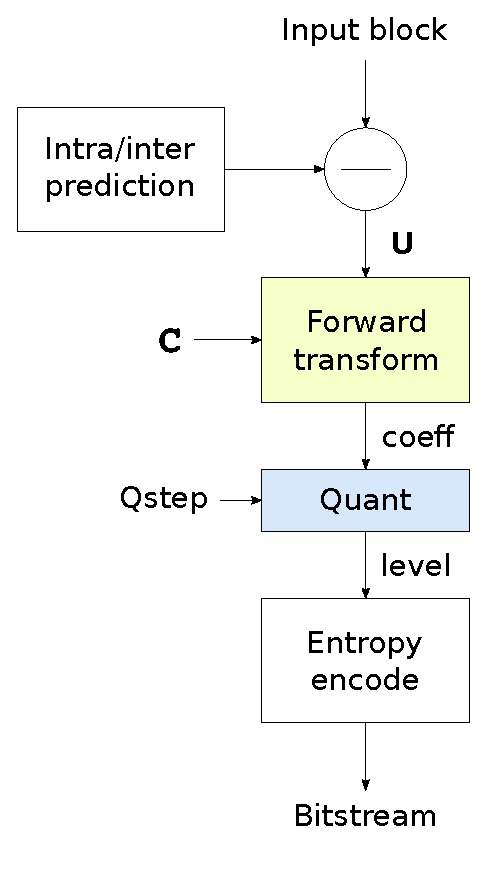
\includegraphics[scale=.66]{Figures/Transf_and_quant_a}}
    &\qquad
    \subfloat[]{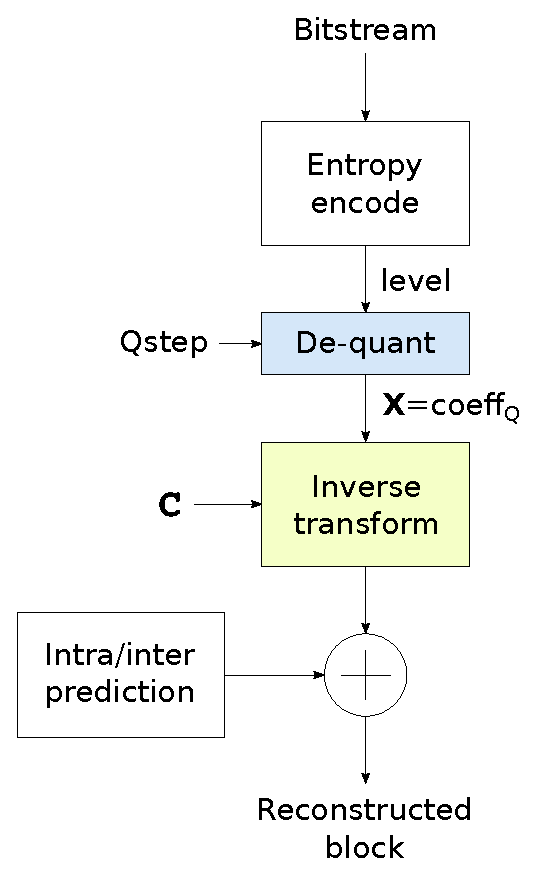
\includegraphics[scale=.66]{Figures/Transf_and_quant_b}}
  \end{tabular}
  \caption{\emph{Data flow} di encoding e decoding.}
\end{figure}
\subsection{Transform}
Tipicamente le trasformate sono delle matrici costruite in modo tale che, in 
assenza di quantizzazione, sommando trasformata e trasformata inversa si 
ottenga un risultato praticamente lossless.
HEVC utilizza due tipologie di trasformate, ovvero quelle derivate dalla DCT e
quelle derivate dalla DST; fornisce inoltre delle matrici precostruite per 
eseguire l'antitrasformata DCT e DST per tutte le possibili dimensioni dei 
blocchi: $4x4$, $8x8$, $16x16$ e $32x32$.
Queste matrici contengono approssimazioni ad interi con precisione finita dei 
coefficienti di trasformazione DCT-II; questo sistema riduce di molto la 
complessità di encoder e decoder, e risolve un problema che era presente in 
H.261, ovvero la deriva dovuta a lievi disallineamenti nella rappresentazione 
fixed point dei coefficienti tra la matrice di trasformazione, costruita 
arbitrariamente dal'implementatore dell'encoder, e quella di antitrasformazione 
fornita dallo standard. \\
Errori di questo tipo si ripercuotono amplificati in ogni immagine successiva, 
costringendo a dover trovare un modo di ovviare al problema (il sopracitato 
H.261 costringeva un aggiornamento periodico del segnale che consisteva in una 
immagine codificata interamente intra).
\subsection{Quantization}
Con ``quantizzazione'' si intende la divisione dei valori trasformati 
utilizzando un passo di quantizzazione $Q_s$ (\emph{quantization step}) definito
 attraverso il parametro di quantizzazione $Q_p$ come segue:
\begin{align*}
Q_s = \left(2^{\frac{1}{6}}\right)^{(Q_p-4)}
\end{align*}
Dalla formula si può notare come una variazione di $1$ per $Q_p$ si traduca in 
una moltiplicazione di $Q_s$ per un fattore $2^{\frac{1}{6}}\approx 1.12$, ovvero 
nell'incremento di $Q_s$ del $12\%$. Una variazione di $6$ si traduce in un 
raddoppiamento di $Q_s$ \\
Si può anche eseguire una quantizzazione \emph{frequency dependent} specificando
 una matrice $w$ con un valore di quantizzazione per ogni frequenza, con un 
risultato che risulta il seguente:
\begin{align*}
q[x][y] = \frac{tc[x][y]}{q[x][y]*Q_s}+offset
\end{align*}
dove $tc$ sono i coefficienti trasformati. \\
Si ottiene una compressione in quanto i valori, una volta quantizzati, verranno 
arrotondati all'intero più vicino. Il fine è quello di portare a 0 il maggior 
numero possibile di coefficienti in modo che la codifica successiva (marcata 
come \emph{Entropy encode}) sia in grado di comprimere al meglio la sequenza in 
uscita; dividendo un intero per un numero più grande il risultato sarà più 
vicino a zero. Tipicamente le matrici di quantizzazione possiedono valori più 
grandi alle basse frequenze e viceversa alle alte, perché il contenuto utile 
per il sistema visivo umano è concentrato alle basse frequenze.

%-------------------------------------------------------------------------------
%       SECTION 5
%-------------------------------------------------------------------------------

\section{In-Loop Filters}
Lo standard ibrido di codifica HEVC scompone i frame attraverso una struttura a 
blocchi per effettuare la compressione; questa suddivisione porta spesso alla 
comparsa di artefatti che danno alle sequenze video un'aspetto quadrettato, 
peggiorandone la qualità visiva. Un esempio tipico di causa della discontinuità 
tra i blocchi è la predizione inter di due blocchi contigui che nel frame
 di riferimento erano distanti, oppure anche la codifica di due blocchi contigui
 con modalità predittive differenti (due intra diversi, una inter e una intra, 
etc.). Per porre rimedio a questi artefatti lo standard HEVC specifica due 
filtraggi: il \emph{deblocking filter} e il \emph{sample adaptive offset} (SAO).
\\ \\
Questi filtraggi sono chiamati \emph{in-loop filters} perché vengono eseguiti 
all'interno dei cicli di encoding/decoding, e i risultati vengono utilizzati 
nei cicli successivi oltre che durante la visualizzazione delle sequenze 
decodificate; in questo modo si trae vantaggio da questa procedura anche durante
 il decoding dei frame successivi, preché le predizioni inter vengono effettuate
 a valle di frame reference di maggiore qualità.
\\ \\
Il \emph{deblocking filter} si occupa di smussare i confini tra due blocchi in 
cui è presente una discontinuità, cercando di lavorare solo su quelle 
introdotte durante la compressione e non quelle originariamente presenti nella 
sequenza. \\
Il SAO, invece, si occupa di ridurre gli artefatti dovuti a trasformazioni e 
quantizzazioni grossolane (chiamati \emph{ringing artifacts}), ed opera 
sull'output del \emph{deblocking filter} in cascata. \\
Visto che i due filtraggi operano su due artefatti diversi, i loro benefici 
sono additivi se eseguiti insieme.
\subsection{Deblocking Filter}
Il \emph{deblocking filter} si applica solo ai confini tra blocchi di tipo CU, 
PU o TU e non al loro interno; durante la codifica  l'encoder considera gruppi 
di quattro vettori di campioni perpendicolari ai confini dei blocchi. 
Specificamente l'encoder esegue alcuni controlli sul primo e sul quarto vettore 
per decidere:
\begin{itemize}
\item Se eseguire il filtraggio o meno;
\item In caso positivo quale filtraggio applicare tra \textbf{normal} e 
\textbf{strong}.
\end{itemize}
Questi semplici controlli misurano un indice di distorsione dei vettori di 
campioni rispetto ad una delle funzioni continue più semplici, ovvero una rampa 
che attraversa il confine \textbf{/*(di che cosa?)*/}. Se questo indice supera 
una certa soglia, che dipende dal passo di quantizzazione $Q_p$ secondo una 
\emph{look-up table}, si esegue il filtraggio.

\begin{figure}[H]
  \captionsetup{justification=raggedright}
  \centering
  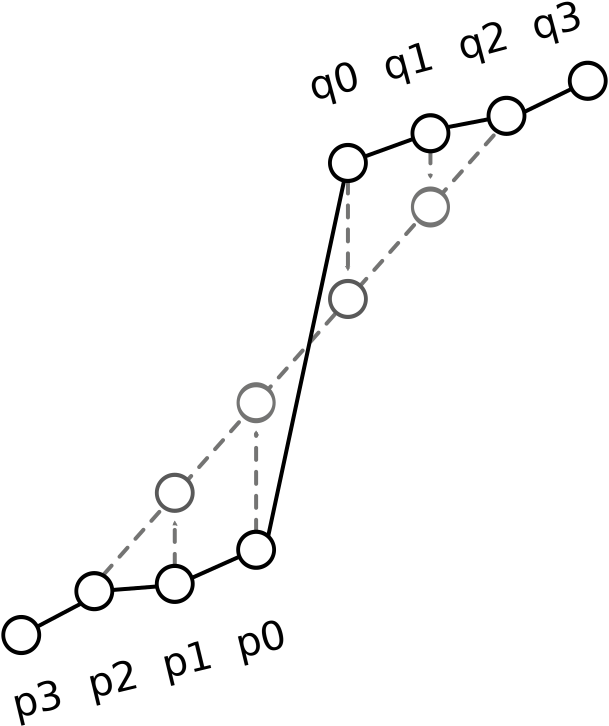
\includegraphics[scale=0.45]{Figures/Deblocking_filter}
    \caption[Filtraggio \emph{deblocking} di tipo \textbf{normal}]
    {Filtraggio \emph{deblocking} di tipo \textbf{normal}: la linea nera mostra
      il confine originale del blocco, la linea grigia tratteggiata quello 
      nuovo}
\end{figure}

L'immagine mostra il risultato di un filtraggio \textbf{normal} eseguito su un 
vettore di 8 campioni, con questi ultimi appartenenti a due blocchi confinanti 
chiamati $P$ e $Q$. \\
In generale, un filtraggio \textbf{normal} può arrivare a modificare fino a due
campioni per lato avvicinandoli alla rampa, come accade nell'immagine.
Il filtraggio \textbf{strong} viene utilizzato nelle aree che racchiudono 
contenuti a bassa frequenza, ovverosia quelle in cui il sistema visivo umano è 
più sensibile alle discontinuità, e consiste in un filtraggio lineare lowpass 
che comprende tre campioni per lato.
\\ \\
Il filtraggio \emph{deblocking} descritto interessa solamente il canale luma, 
dal momento che per i canali chroma si opera un filtraggio analogo ma più 
grossolano, in cui vengono eseguiti molti meno controlli e vengono considerati 
meno campioni: ciò permette di ridurre la complessità dell'encoder a fronte di 
una bassa perdita di qualità, sempre considerando il fatto che i canali chroma 
sono meno importanti per il sistema visivo umano.
\subsection{Sample Adaptive Offset - SAO}
